\documentclass{beamer}
\usepackage{pgffor,pgfmath}
\usepackage{lipsum}
\usepackage{multicol}
\usetheme{ucla}
\usepackage{graphicx}
\usepackage{listings}
\usepackage{verbatim}
\usepackage{tikz}
\linespread{1.5}
\usepackage{comment}

\usepackage{amsmath, amsthm, amssymb, latexsym}

%\newtheorem{definition}{Definition}

\title{Lecture 6}
\author{Charles Rambo}
\institute{UCLA Anderson School of Management}
\date{2023}
\location{Los Angeles, California}

% Turn on slide numbers:
\showSlideNumber{}

\AtBeginSection[]
{
    \begin{frame}
        \frametitle{Table of Contents}
        \tableofcontents[currentsection]
    \end{frame}
}


\begin{document}

\insertTitleSlide


\section{Partial Derivatives}

\begin{frame}
\frametitle{Partial Derivatives}
{\small 
\begin{Definition}
Suppose we have $f:\mathbb{R}^n \to \mathbb{R}$. Then the {\bf partial derivative} of $f$ with respect to $x_i$ is
$$
\frac{\partial f}{\partial x_i} = \lim_{h\to 0} \frac{f(x_1, x_2,\ldots, x_i + h,\ldots, x_n) - f(x_1, x_2,\ldots, x_n)}{h}.
$$
The most common case is $f:\mathbb{R}^2\to \mathbb{R}$ such that $z = f(x, y)$. Then the two partials are
$$
f_x(x, y) = \frac{\partial z}{\partial x} = \lim_{h\to 0 } \frac{f(x + h, y) - f(x, y)}{h}
$$
and
$$
f_y(x, y) = \frac{\partial z}{\partial y} = \lim_{h\to 0 } \frac{f(x, y + h) - f(x, y)}{h}.
$$
\end{Definition}
}
\end{frame}

\begin{frame}
\frametitle{Clairaut's Theorem}

\begin{Theorem}[Clairaut]
Suppose $f$ is defined on a disk $D$ that contains the point $(a, b)$. If the functions $f_{xy}$ and $f_{yx}$ are both continuous on $D$, then
$$
f_{xy}(a, b) = f_{yx}(a, b).
$$
\end{Theorem}

\end{frame}

\begin{frame}
\frametitle{Difference Approximation}

\begin{Theorem}
Suppose $f_x$ and $f_y$ exist on a rectangular region $R$ with sides parallel to the axes and containing the points $(a, b)$ and $(a + \Delta x, b + \Delta y)$. Suppose $f_x$ and $f_y$ are continuous at the point $(a, b)$, and let
$$
\Delta z = f(a + \Delta x, b + \Delta y) - f(a, b).
$$
Then
$$
\Delta z = f_x(a, b)\Delta x + f_y(a, b)\Delta y + \varepsilon_1\Delta x + \varepsilon_2\Delta y
$$
where $\varepsilon_1,\varepsilon_2\to 0$ as $\Delta x,\Delta y\to 0$.

\end{Theorem}

\end{frame}

\begin{frame}[t]
\frametitle{Example}
\begin{Example}
Suppose $f(x, y, z) = \sqrt{xyz}$. Approximate $f(3.9, 4.2, 3.9)$.
\end{Example}

\end{frame}

\begin{frame}
\frametitle{The Chain Rule}

Suppose $u$ is a differentiable function of $n$ variables $x_1, x_2,\ldots, x_n$ and each $x_j$ is a function of the $m$ variables $t_1, t_2,\ldots, t_m$ such that the partial derivate $\frac{\partial x_j}{\partial t_i}$ exists each for all $i$ and $j$. Then $u$ is a function of $t_1, t_2,\ldots, t_m$ and
$$
\frac{\partial u}{\partial t_i} = \frac{\partial u}{\partial x_1}\frac{\partial x_1}{\partial t_i} + \frac{\partial u}{\partial x_2}\frac{\partial x_2}{\partial t_i} + \ldots + \frac{\partial u}{\partial x_n}\frac{\partial x_n}{\partial t_i}
$$
for any $i$.

\end{frame}

\begin{frame}[t]
\frametitle{Chain Rule Example}
\begin{Example}
Consider the Black-Scholes differential equation
$$
\frac{\partial V}{\partial t} + \frac{\sigma^2}{2} S^2 \frac{\partial^2 V}{\partial S^2} + r S \frac{\partial V}{\partial S} = r V.
$$
Rewrite the differential equation using the substitution $z = \ln S$.
\end{Example}

\end{frame}

\begin{frame}
\frametitle{Implicit Differentiation}
Suppose that $F(x, y) = 0$ and $y = f(x)$. Then
$$
\frac{\partial F}{\partial x} + \frac{\partial F}{\partial y} \frac{d y}{d x} = 0.
$$
So,
$$
\frac{dy}{dx} = -\frac{\frac{\partial F}{\partial x}}{\frac{\partial F}{\partial y}}= - \frac{F_x}{F_y}
$$
as long as $\frac{\partial F}{\partial x}$ is continuous and $\frac{\partial F}{\partial y}$ is both continuous and nonzero.
\end{frame}

\begin{frame}[t]
\frametitle{Implicit Differentiation Example}
\begin{Example}
Find $\frac{dy}{dx}$ if $x^3 + y^3 = 6xy$.
\end{Example}
\end{frame}

\begin{frame}
\frametitle{Gradient Vector}
Let's introduce new notation. Suppose $x\in\mathbb{R}^n$. Define
$$
\nabla f(x) = \left(\frac{\partial f}{\partial x_1}, \frac{\partial f}{\partial x_2},\ldots, \frac{\partial f}{\partial x_n}\right).
$$
\end{frame}

\subsection{Gradient Vector}
\begin{frame}
\frametitle{Space Curve}
A curve in $\mathbb{R}^n$ can be defined in terms of a vector valued function $r$, where $r:I\to\mathbb{R}^n$ and $I$ is some subset of $\mathbb{R}$. 

For example, consider $r:[0, 2\pi)\to\mathbb{R}^2$ such that $r: t \mapsto \left(\cos t, \sin t\right)$. This defines a circle oriented counterclockwise in $\mathbb{R}^2$.
\begin{center}
\begin{tikzpicture}[scale = 1.5]
\draw[->] (-1.25, 0) -- (1.7, 0) node[right] {$x$};
\draw[->] (0, -1.25) -- (0, 1.25) node[above] {$y$};

\draw[blue] (0, 0) circle (1);


\node[blue] at (1,0) {.};
\node[blue] at (0,1) {.};
\node[blue] at (-1,0) {.};
\node[blue] at (0,-1) {.};
	
\draw[->, blue] (1, 0) -- (1, 0.1) node[right] {$t = 0$};
\draw[->, blue] (0, 1) -- (-0.1, 1) node[above left] {$t = \frac{\pi}{2}$};
\draw[->, blue] (-1, 0) -- (-1, -0.1) node[below left] {$t = \pi$};
\draw[->, blue] (0, -1) -- (0.1, -1) node[below right] {$t = \frac{3\pi}{2}$};

\end{tikzpicture}

\end{center}
\end{frame} 

\begin{frame}[t]
\frametitle{Derivatives of Space Curves}
The derivative of $r:I\to\mathbb{R}^n$ is defined to be
$$
r\; '(t) =\lim_{h\to 0} \frac{r(t + h) - r(t)}{h}.
$$
The derivative is tangent to the curve described by $r$.
\end{frame}

\begin{frame}
\frametitle{Gradient Vector Orthogonal to Surface}
\small 
Suppose that we have a surface defined by $F(x) = k$ where $x$ is in $\mathbb{R}^n$. Consider any curve defined by $r: I\to \mathbb{R}^n$. Then we have the value of the function at $r(t)$ is
$$
F(r(t)) = k.
$$
The chain rule implies
$$
\nabla F(r(t))\bullet r\ '(t) = 0.
$$
The vector $r\; '(t)$ is parallel to the surface. Hence, $\nabla F(r(t))$ is orthogonal. Since $r$ was arbitrary, we must have $\nabla F(x)$ is orthogonal to $F(x) = k$.
\end{frame}

\begin{frame}
\frametitle{Gradient Vector Example}

Consider $F(x, y) = x + y = 1$. Then $\nabla F = (1, 1)$. We can see this vector is orthogonal to our line (or ``surface" to use the more general term).
\begin{center}
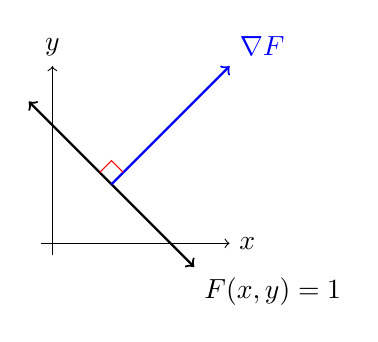
\begin{tikzpicture}[scale = 1.5]

\draw[->] (-0.1, 0) -- (1.5, 0) node[right] {$x$};
\draw[->] (0, -0.1) -- (0, 1.5) node[above] {$y$};

\draw[<->, thick] (-0.2, 1.2) -- (1.2, -0.2) node[below right] {$F(x, y) = 1$};

\draw[->, blue, thick] (0.5, 0.5) -- (1.5, 1.5) node[above right] {$\nabla F$};

\draw[red] (0.4, 0.6) -- (0.5, 0.7) -- (0.6, 0.6);
\end{tikzpicture}
\end{center}
\end{frame}


\section{Maximum and Minimum Values}

\begin{frame}
\frametitle{Local Maximum and Minimum}

\begin{Definition}
A function of two variables has a {\bf local maximum} at $(a, b)$ if $f(x, y)\leq f(a, b)$ for all points $(x, y)$ in some disk with center $(a, b)$. The number $f(a, b)$ is called a {\bf local maximum value}, if $f(x, y) \geq f(a, b)$ for all $(x, y)$ in such a disk, $f(a, b)$ is a {\bf local minimum value}.
\end{Definition}

\begin{Theorem}
If $f$ has a local extremum at $(a, b)$ and the first-order partial derivatives of $f$ exist there, then $f_x(a, b) = f_y(a, b) = 0$.
\end{Theorem}

\end{frame}

\subsection{Second Derivatives Test}

\begin{frame}
\frametitle{Second Derivatives Test}
Suppose the second partial derivatives of $f$ are continuous in a disk with center $(a, b)$, and suppose that $f_x(a, b) = f_y(a, b) = 0$. Let
$$
D = \left|\begin{array}{c c} f_{xx}(a, b)	&	f_{xy}(a, b)\\ f_{yx}(a, b)	&	f_{yy}(a, b)\end{array}\right|.
$$
\begin{enumerate}
\item[(a)] If $D >0$ and $f_{xx} (a, b) > 0$, then $f(a,b)$ is a local minimum.
\item[(b)] If $D > 0$ and $f_{xx}(a, b) < 0$, then $f(a, b)$ is a local maximum.
\item[(c)] If $D < 0$, then $f(a, b)$ is not a local extremum.
\item[(d)] If $D = 0$, then the test fails.
\end{enumerate}

\end{frame}


\begin{frame}[t]
\frametitle{Second Derivatives Test Example}
\begin{Example}
Find the shortest distance from the point $(1, 0, -2)$ to the plane $x + 2y + z = 4$.
\end{Example}
\end{frame}

\begin{frame}[fragile]
\frametitle{Minimization Python Example}
\small

\begin{Example}
Use Python to verify the previous example.
\end{Example}

{\bf Solution.}
{
\linespread{0.8}
\tiny
\begin{verbatim*}
import numpy as np
from scipy.optimize import minimize

# Define function
def distance(pt):
    
    # Get the x- and y-values
    x, y = pt[0], pt[1]
    
    # Define z 
    z = 4 - x - 2 * y
    
    return np.sqrt((x - 1)**2 + y**2 + (z + 2)**2)

# Get the result   
minimize(distance, x0 = [0, 0]) 

# Another option is to use the constraint x + 2y + z - 4 = 0 and optimize with three variables 
\end{verbatim*}
}

\end{frame}

\begin{frame}
\frametitle{Minimization Python Result}
Note that
$$
\frac{11}{6} \approx 1.83,\qquad \frac{5}{3} \approx 1.67\qquad\text{and}\qquad \frac{5\sqrt{6}}{6}\approx 2.04
$$
\begin{center}
\includegraphics[scale = 0.4]{ex8.png}
\end{center}
\end{frame}

\begin{frame}
\frametitle{Extreme Value Theorem for Functions of Two Variables}
\begin{Theorem}
If $f$ is continuous on a closed and bounded set $D$ in $\mathbb{R}^2$, then $f$ attains an absolute maximum value $f(x_1, y_1)$ and an absolute minimum value $f(x_2, y_2)$ at some points $(x_1, y_1)$ and $(x_2, y_2)$ in $D$.
\end{Theorem}
\end{frame}

\subsection{Global Optimization}

\begin{frame}[t]
\frametitle{Global Optimization}
\begin{Example}
Find the absolute maximum and minimum values of $f(x, y) = 5 - 3x + 4y$ on the triangular region with vertices $(0, 0)$, $(4, 0)$, $(4, 5)$.
\end{Example}
\end{frame}

\begin{frame}
\frametitle{Global Optimization in Python}
\tiny
There are many global optimization techniques in Python. However, they tend to be slow and not particularly effective on functions that aren't convex or concave. See the \href{https://docs.scipy.org/doc/scipy/reference/optimize.html}{SciPy documentation} for more details. 
\begin{center}
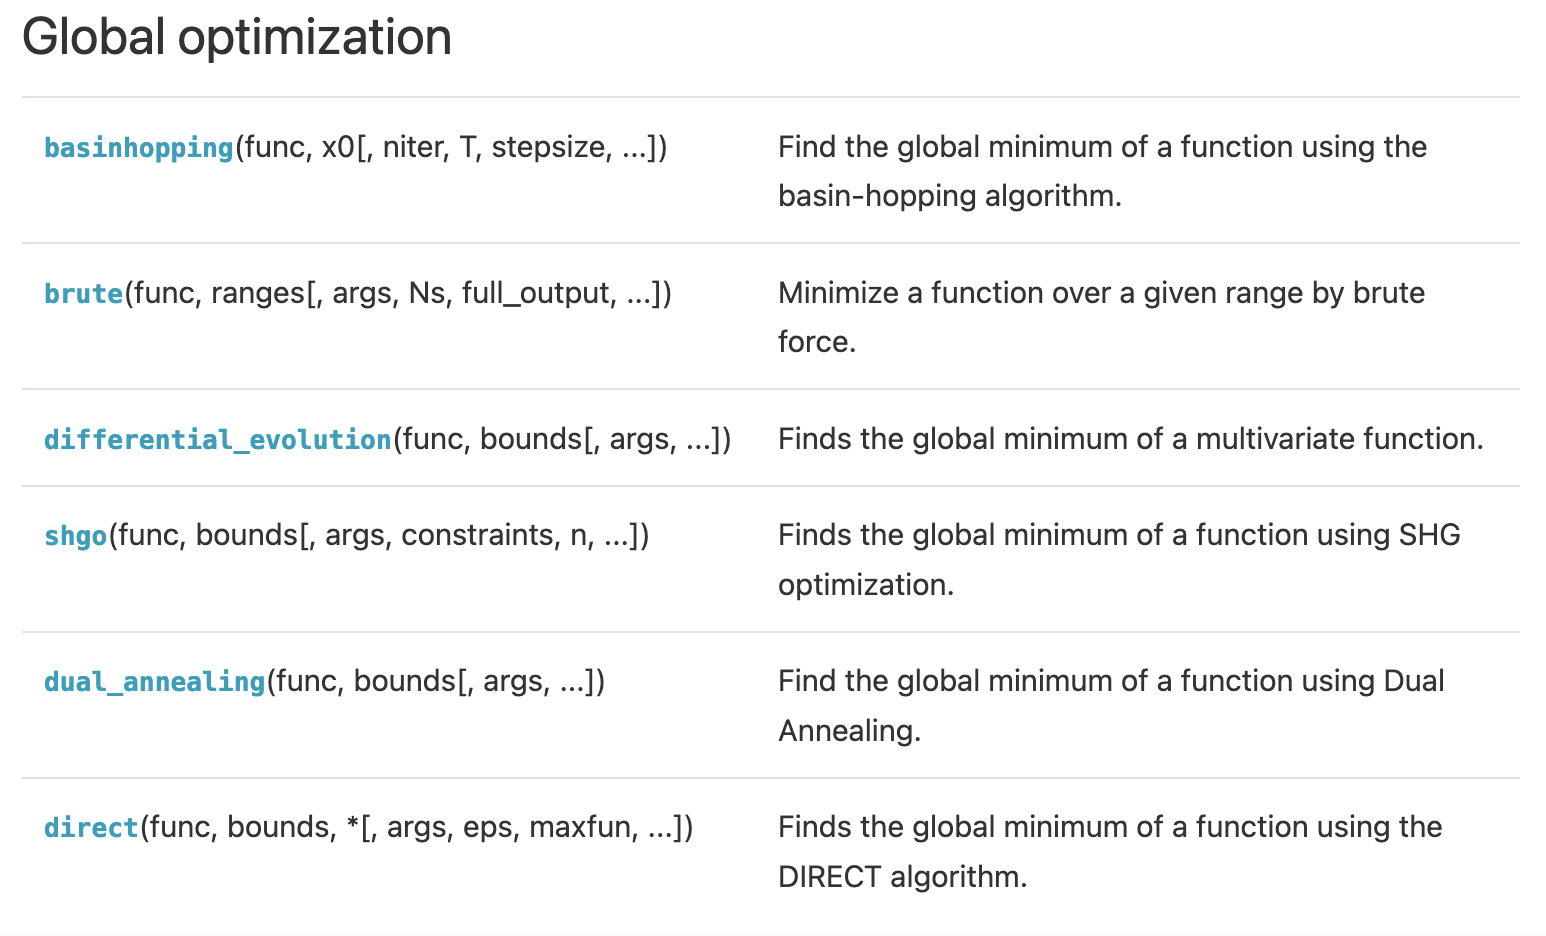
\includegraphics[scale = 0.3]{global.png}
\end{center}
\end{frame}

\section{Lagrange Multipliers}

\begin{frame}
\frametitle{Lagrange Multipliers}
For $x\in \mathbb{R}^n$, consider $f(x)$ subject to $g(x) = k$. If extrema exist, they satisfy the equation
$$
\nabla f(x) = \lambda \nabla g(x).
$$
for some $\lambda$ in $\mathbb{R}$.
\end{frame}


\begin{frame}
\frametitle{Lagrange Multipliers Picture}
\begin{center}
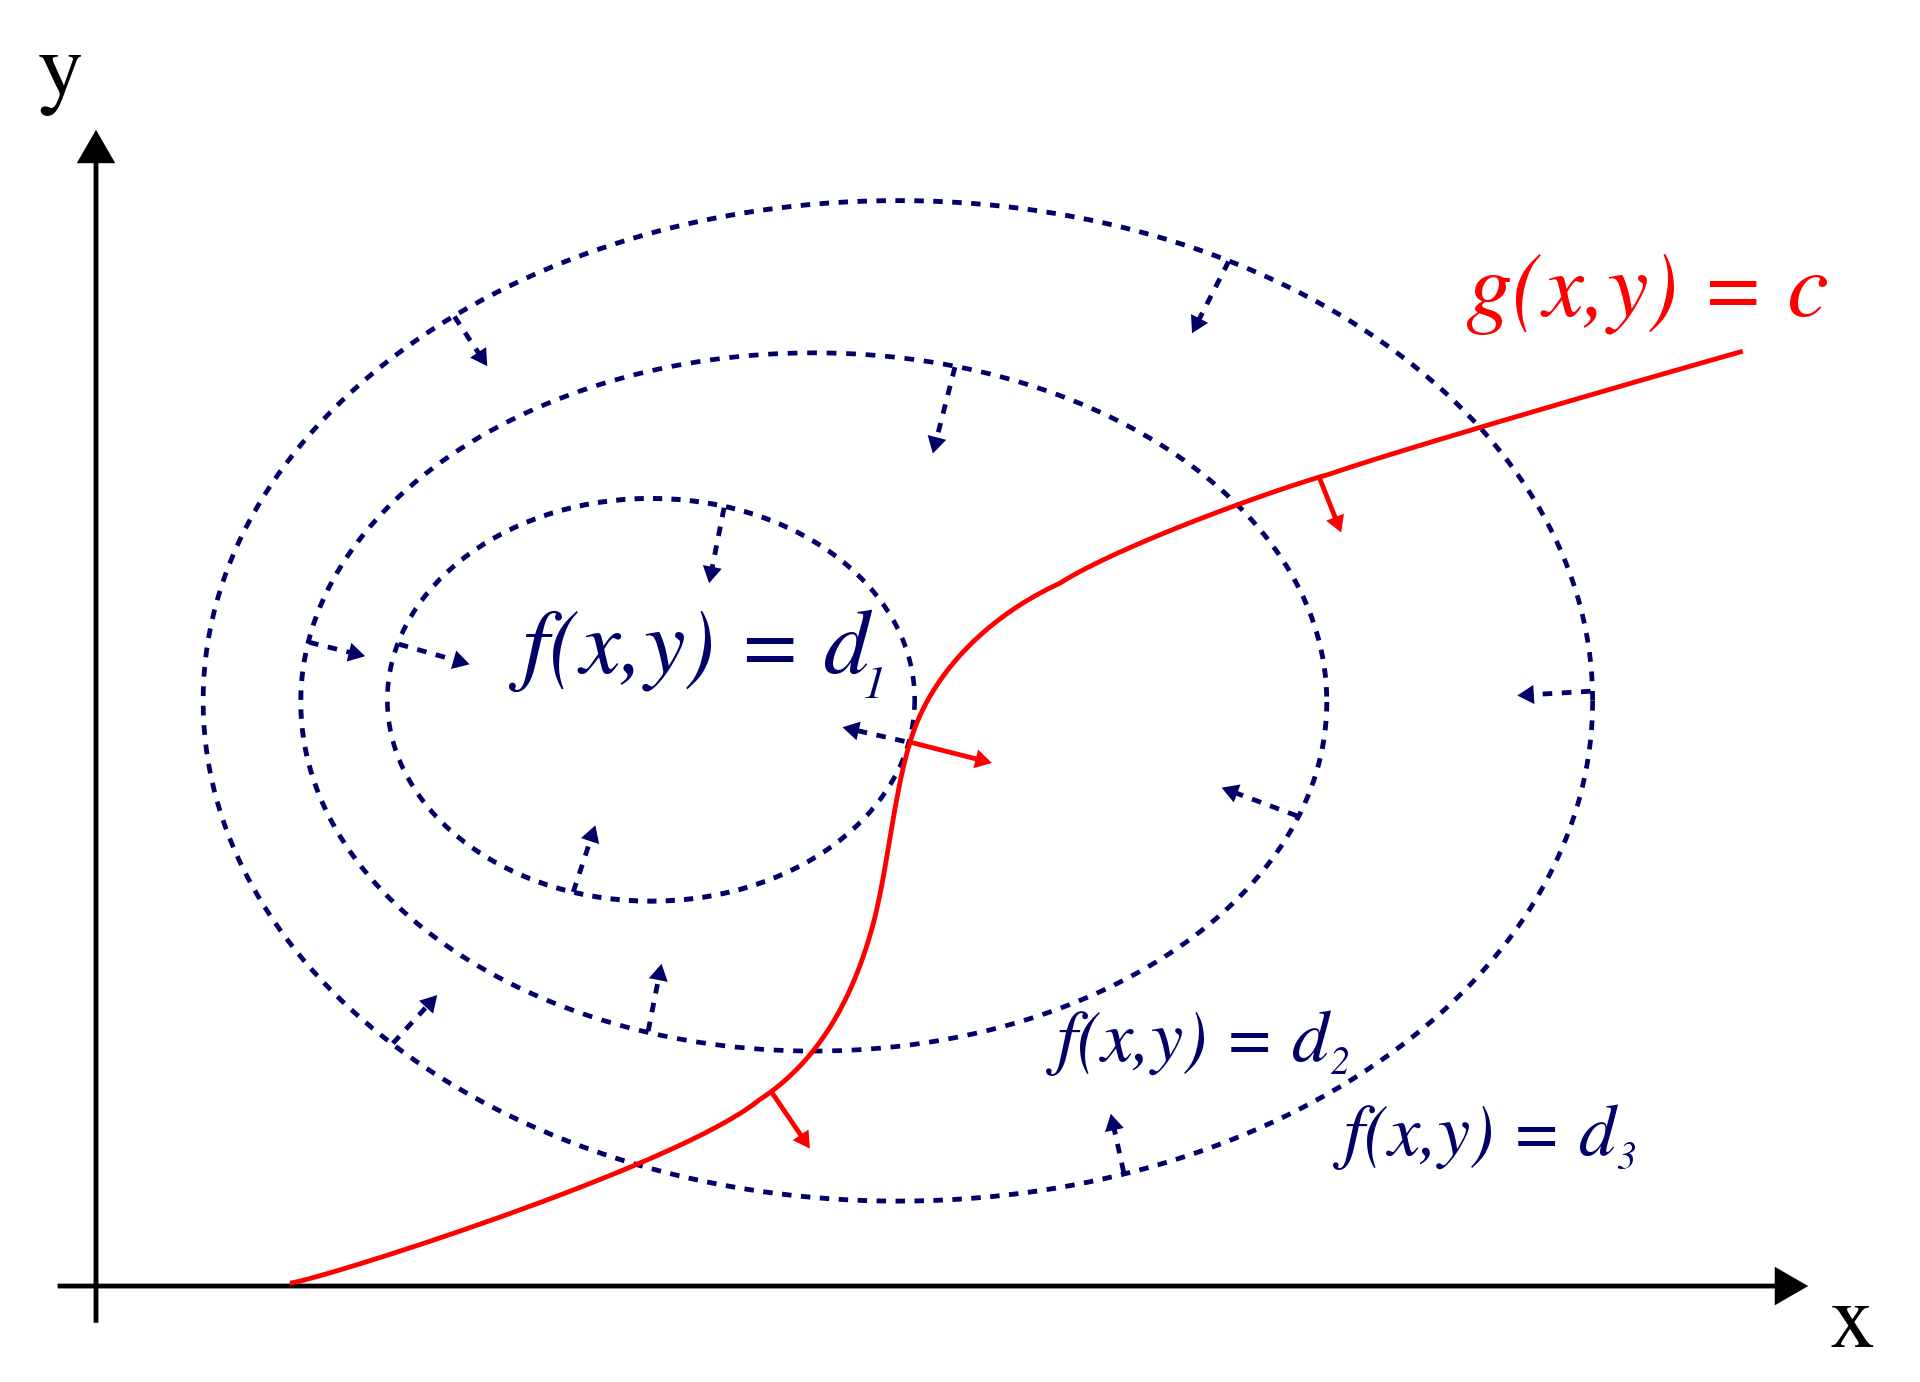
\includegraphics[scale = 0.1]{LagrangeMultipliers.png}
\end{center}
\end{frame}

\begin{frame}[t]
\frametitle{Lagrange Multipliers Example}
\begin{Example}
Find the shortest distance from the point $(1, 0, -2)$ to the plane $x + 2y + z = 4$.
\end{Example}
\end{frame}

\section{Multiple Integrals}

\begin{frame}
\frametitle{Construction of Double Integral}
\tiny
Consider $f:\mathbb{R}^2\to\mathbb{R}$ and define the closed region
$$
R = [a, b]\times [c, d] = \{(x, y)\in\mathbb{R}^2: a\leq x\leq b,\ c\leq y\leq d\}.
$$
Consider partition $P$ of $R$ into subrectangles $R_{ij} = [x_{i - 1}, x_i]\times [y_{i - 1}, y_i]$, where
\begin{align*}
a &= x_0 \leq x_1 < \ldots < x_m = b\\
c &= y_0 \leq y_1 < \ldots < y_n = d\\
\end{align*}
Select $(s_{ij}, t_{ij})$ from $R_{ij}$. The area of $R_{ij}$ is $\Delta A_{ij} = \Delta x_i\Delta y_j$. Define the mesh $\|P\| = \max_{i, j}\{\Delta A_{ij}\}$. Then
$$
\iint_R f(x, y)\ dA = \lim_{\|P\|\to 0} \sum_{i = 1}^m\sum_{j = 1}^n f(s_{ij}, t_{ij})\ \Delta A_{ij}
$$
whenever the limit exists.
\end{frame}

\begin{frame}[t]
\frametitle{Double Integral Example}
\begin{Example}
Calculate $\displaystyle\iint_{[0,1]\times[0, 1]} xy^2\ dA$. Use a uniform partition with $n^2$ subrectangles $R_{ij}$, and the upper right point of $R_{ij}$ for $(s_{ij}, t_{ij})$.
\end{Example}
\end{frame}

\begin{frame}[fragile]
\frametitle{Double Integral Python Example}
\small
\begin{Example}
Use \texttt{scipy.integrate.dblquad} to verify the previous result for $\displaystyle\iint_{[0,1]\times[0, 1]} xy^2\ dA$.
\end{Example}
{\bf Solution.}
{
\tiny
\linespread{0.8}
\begin{verbatim*}
import numpy as np
from scipy.integrate import dblquad

# Define f
f = lambda y, x: x * y**2

# Integrate
dblquad(f, 0, 1, 0, 1)[0]
\end{verbatim*}
}
The output is \texttt{0.16666666666666669} which agrees with our previous result. 

\end{frame}

\begin{frame}
\frametitle{Fubini's Theorem}
\begin{Theorem}[Fubini]
Consider $R = [a, b]\times [c, d]$ and define
$$
A_1(x) = \int_c^d f(x, y)\ dy\qquad A_2(y) = \int_a^b f(x, y)\ dx.
$$
Then
$$
\iint_R f(x, y)\ da = \int_a^b A_1(x)\ dx = \int_c^d A_2(y)\ dy.
$$
\end{Theorem}
\end{frame}

\begin{frame}[t]
\frametitle{Fubini's Theorem Example}
\begin{Example}
Evaluate $\displaystyle\iint_R y\sin(xy)\ dA$, where $R = [1, 2]\times [0, \pi]$.
\end{Example}

\end{frame}

\begin{frame}
\frametitle{Integral over General Region}
To calculate
$$
\iint_D f(x, y)\ dA
$$
where $D$ isn't a rectangle, simply choose rectangle $R$ which contains $D$ and define
$$
F(x, y) = \begin{cases} f(x, y),	&	(x, y)\in D\\ 0,	&	(x,y)\in R\setminus D.\end{cases}
$$
\end{frame}

\begin{frame}[t]
\frametitle{Integral of General  Region}
\begin{Example}
Compute $\displaystyle\iint_D ye^x\ dA$, where $D$ is the triangular region with verticies $(0, 0)$, $(2, 4)$, and $(6, 0)$.
\end{Example}

\end{frame}

\subsection{Change of Variables}

\begin{frame}
\frametitle{Jacobian}
\begin{Definition}
The {\bf Jacobian} of the transformation given by $x = g(u, v)$ and $y = h(u, v)$ is
$$
J = \left(\begin{array}{c c} \frac{\partial x}{\partial u}	&	\frac{\partial x}{\partial v}\\ \frac{\partial y}{\partial u} &	\frac{\partial y}{\partial v}\end{array}\right).
$$
\end{Definition} 

\end{frame}

\begin{frame}
\frametitle{Change of Variables}
Suppose that we have a one-to-one transformation with continuous partial derivatives that maps the $uv$-plane to the $xy$-plane, and in particular the region $S$ to $D$. Then
$$
\iint_D f(x, y)\ dxdy = \iint_S f\left(x(u, v), y(u, v)\right)\left|\text{det}(J)\right|\ dudv.
$$

\end{frame}

\begin{frame}[t]
\frametitle{Change of Variables Example}
\begin{Example}
$\displaystyle\int_{-\infty}^{\infty} e^{-x^2/2}\ dx = $
\end{Example}

\end{frame}

\begin{frame}
\frametitle{Jacobian on YouTube}
\small
Watch the Mathemaniac video about the Jacobian on YouTube (\url{https://youtu.be/wCZ1VEmVjVo}).
\begin{center}

\includegraphics[scale = 0.3]{Mathemaniac.png}
\end{center}
\end{frame}



\end{document}